\begin{pastexam}[label={px:gw3-113-ds-04}]{關務三等資訊處理 113 年 第四題}
（申論；15 分）

有一棵二元樹（binary tree）利用一維陣列來存放其節點，假設樹根（root）存放在索引（index）為 1 的位置，若有一節點 i 存放在
索引為 1024 的位置，請問該節點 i 的父節點存於陣列的那個位置，其索引為何？若節點 i 有一右子節點 j，請問節點 j 存於陣列的
那個位置，其索引為何？用一維陣列存放二元樹，最浪費陣列空間的二元樹是那一種？請畫出並詳細說明。（15 分）
\end{pastexam}

\begin{pastsoln}
答案：父節點在索引 $512$；右子節點 j 在索引 $2049$。 最浪費空間的是右斜樹（每個節點只有右子節點），$k$ 個節點要用到
$2^{k} - 1$ 格。

\textbf{陣列表示}（資結書第~7.2~節）：把樹當成完整二元樹，由上而下、由左而右從 $1$ 編號，節點放在自己的編號上。 節點 $x$
的左子節點是 $2x$、右子節點是 $2x + 1$、父節點是 $\lfloor x/2 \rfloor$。 （第 $d$ 層，根是第 $0$ 層，編號從 $2^{d}$ 到
$2^{d+1} - 1$；某節點前面同一層的每個節點都有兩個子位置，所以子節點的編號是 $2x$、$2x + 1$。）

\begin{itemize}
\item 節點 i 在 $1024$：父節點 $\lfloor 1024 / 2 \rfloor = 512$。 $1024$ 是偶數，所以 i 是 $512$ 號節點的\textbf{左}子節點。
\item i 的右子節點 j 在 $2 \times 1024 + 1 = 2049$。
\item 順帶一提，$1024 = 2^{10}$，i 是第 $10$ 層（根是第 $0$ 層）最左邊的節點，從根一路往左走 $10$ 步。
\end{itemize}

\textbf{最浪費空間的樹：右斜樹。} 陣列大小由用到的最大編號決定。 $k$ 個節點、高度 $k$ 的斜樹（每個節點只有一個子節點）
最深，而一路往右走時編號長得最快：
\[
1 \to 3 \to 7 \to 15 \to \cdots \to 2^{k} - 1.
\]
所以 $k$ 個節點的右斜樹要開 $2^{k} - 1$ 格，只用了其中 $k$ 格，浪費 $2^{k} - 1 - k$ 格。 這是所有 $k$ 個節點的二元樹中最大
編號的上限：高度 $k$ 的樹最大編號不超過 $2^{k} - 1$（第 $k - 1$ 層最右邊），右斜樹正好達到。 左斜樹編號是
$1, 2, 4, \dots, 2^{k-1}$，要 $2^{k-1}$ 格，約浪費一半，比右斜樹少；完整二元樹則一格都不浪費。

例如 $k = 4$ 的右斜樹：
\begin{center}
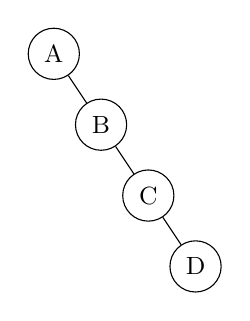
\begin{tikzpicture}[every node/.style={circle,draw,minimum size=6.5mm,inner sep=0pt,font=\small},
  level distance=9mm, sibling distance=12mm]
\node {A}
  child[missing]
  child {node {B} child[missing] child {node {C} child[missing] child {node {D}}}};
\end{tikzpicture}
\qquad
\begin{tabular}[b]{|c|*{15}{c|}}
\hline
1 & 2 & 3 & 4 & 5 & 6 & 7 & 8 & 9 & 10 & 11 & 12 & 13 & 14 & 15 \\ \hline
A & & B & & & & C & & & & & & & & D \\ \hline
\end{tabular}
\end{center}
$15$ 格只用了 $4$ 格。 $k = 20$ 時要 $2^{20} - 1 \approx 10^{6}$ 格卻只存 $20$ 個節點，所以斜樹或很不平衡的樹應該改用鏈結
表示（每個節點用左、右兩個指標）。
\end{pastsoln}
